\documentclass[10pt]{article}

\usepackage{../pplmanual}
%%% Commonly Needed packages
\usepackage{graphicx,color,calc}
\usepackage{fancyvrb}
\usepackage{makeidx}
\usepackage{alltt}
\usepackage[linkbordercolor=(0 0 1),citebordercolor=(0 1 0)]{hyperref}
%%\usepackage{xspace} <- creates problems with other hyperlink packages like "html"

%%% Commands for uniform looks of C++, Charm++, and Projections
\newcommand{\CC}{C\hbox{++}}
\newcommand{\emCC}{C\hbox{\em++}}
\newcommand{\charmpp}{\textsc{Charm++}}
\newcommand{\charmc}{\texttt{charmc}}
\newcommand{\projections}{\textsc{Projections}}
\newcommand{\converse}{\textsc{Converse}}
\newcommand{\ampi}{\textsc{AMPI}}
\newcommand{\tempo}{\textsc{TeMPO}}
\newcommand{\irecv}{\textsl{iRecv}}
\newcommand{\sdag}{\textsl{Structured Dagger}}
\newcommand{\jade}{Jade}

%%% Commands to produce margin symbols
\newcommand{\new}{\marginpar{\fbox{\bf$\mathcal{NEW}$}}}
\newcommand{\important}{\marginpar{\fbox{\bf\Huge !}}}
\newcommand{\experimental}{\marginpar{\fbox{\bf\Huge $\beta$}}}

%%% Commands for manual elements
\newcommand{\zap}[1]{ }
\newcommand{\function}[1]{{\noindent{\textsf{#1}}\\}}
\newcommand{\cmd}[1]{{\noindent{\textsf{#1}}\\}}
\newcommand{\args}[1]{\hspace*{2em}{\texttt{#1}}\\}
\newcommand{\prototype}[1]{\vspace{0.2in}\index{#1}}
\newcommand{\param}[1]{{\texttt{#1}}}
\newcommand{\kw}[1]{{\textsf{#1}\index{#1}}}
\newcommand{\uw}[1]{{\textsl{#1}}}
\newcommand{\desc}[1]{\indent{#1}}
\newcommand{\note}[1]{(\textbf{Note:} #1)}
\newcommand{\term}[1]{{\bf #1}\index{#1}}

\makeindex


\begin{document}

%\maketitle
\begin{titlepage}
 \begin{flushright}
   {\Large
     Parallel Programming Laboratory\\
     University of Illinois at Urbana-Champaign\\
   }
 \end{flushright}
 \rule{\textwidth}{3pt}
 \vspace{\fill}
 \begin{flushright}
   \textsf{\Huge POSE User and Reference Manual \\}
 \end{flushright}
 \vspace{\fill}
 {\small POSE software and this manual are entirely the fault of Terry
L. Wilmarth.  Credit for Charm++ is due to the developers, past and
present, at the Parallel Programming Laboratory ({\tt
http://charm.cs.uiuc.edu}).  Questions or comments on POSE or this
manual can be directed to Terry at {\tt wilmarth@cse.uiuc.edu}.
} \\
 \rule{\textwidth}{3pt}
\end{titlepage}

\tableofcontents
\newpage


\section{About POSE}

POSE (Parallel Object-oriented Simulation Environment) is a tool for
parallel discrete event simulation based on Charm++.  You should have
a background in object-oriented programming (preferably C++), know the
basic principles behind discrete event simulation, and be familiar
with the basic syntax of Charm++.  

POSE uses the approach of message-driven execution of Charm++, but
adds the element of discrete timestamps, to control when in simulated
time, a message is executed.

Users may choose synchronization strategies (conservative or
optimistic) on a per class basis, depending on the desired behavior of
the object. 


\section{Developing a model in POSE}

Modelling a system in POSE is similar to how you would model in C++ or
any OOP language.  Objects are entities that hold data, and have a
fixed set of operations that can be performed on them (methods).

Charm++ provides the parallelism we desire, but the model does not
differ dramatically from C++.  The primary difference is that objects
may exist on a set of processors, and so invoking methods on them
requires communication via messages. 

POSE adds to Charm++ by putting timestamps on method invocations
(events), and executing events in timestamp order to preserve the
validity of the global state.

\begin{figure}[h]
\begin{center}
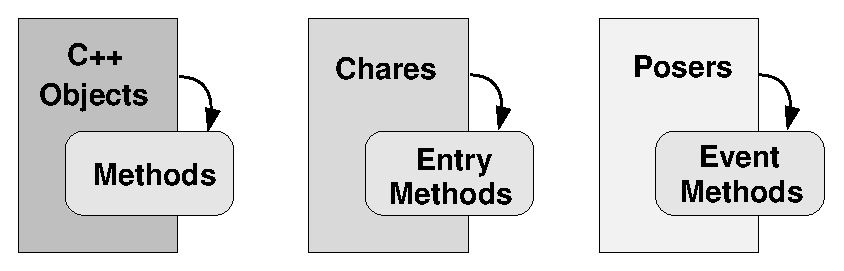
\includegraphics[width=4in]{oopdes}
\end{center}
\caption{Object-Method relationship in C++, Charm++ and POSE.}
\label{fig:oopdes}
\end{figure}

Thus we can see that developing a model in POSE involves identifying
the entities we wish to model, determining how they communicate,
developing a C++ model, accounting for the parallelism of objects by
creating messages for the Charm++ version, and finally, providing the
proper event timing info for the system you wish to simulate.

\section{Example: Industrial Process Simulation}

We consider the problem of modelling an industrial process.  

Fiddler's Widgets Inc. is doing a booming business and has decided to
expand.  They currently have a single automated assembly line and
would like to add a second.  This addition will involve many
decisions.  The original assembly line consists of older, less
efficient, but less expensive equipment.  For the new assembly line,
they have the option of purchasing new state-of-the-art equipment, or
the less expensive earlier model.  They would also like to know,
should they choose to purchase the newer model equipment, would it
also pay off to replace the older equipment on the original assembly
line.

The original assembly line consists of:

\begin{enumerate}
\item A Generator/Dispatcher unit which generates "jobs" (incomplete
versions of the product made by Fiddler's Widgets) of varying
complexity at a rate of one per second. 
\item A Resource/Component Unit which completes the job in a two-phase
process.  The Resource part of the unit is known to breakdown
approximately once a week, takes nearly an hour to fix, and greatly
reduces the number of widgets produced in a 8 hour shift.  In
addition, approximately 2\% of the widgets produced have errors. The
Component part of the unit is capable of detecting these errors and
routing the faulty widget to a junkbin.
\end{enumerate}

The machine is capable of producing ~656 widgets during an eight-hour
shift. Each widget earns the company \$4.00 in profit.  The cost of running the
original assembly line for an eight-hour shift breaks down as follows:

\begin{verbatim}
COSTS:
1) Raw material cost:    $ 167.25  ($0.25 per widget)  
2) Power consumption:    $ 143.97
3) Employee supervision: $ 640.00  (4 employees @ $20/hr)
4) Machine maintenance:  $  33.42  ($234.95 over a week)
   TOTAL:                $ 984.64

PROFIT:
1) Widgets               $2676.00  (669 widgets @ $4 each)

LOSSES:
1) Loss to errors:       $  52.00  (2% = approx. 13)
2) Loss to breakdowns:   $  47.79  (1/7 of profit per hour)
   TOTAL:                $  99.79

NET: $2676.00 - $984.64 - $99.79 = $1591.57

PURCHASE COSTS:
Generator/Dispatcher: $ 999
Resource/Component:   $2150
\end{verbatim}


\begin{figure}[ht]
\begin{center}
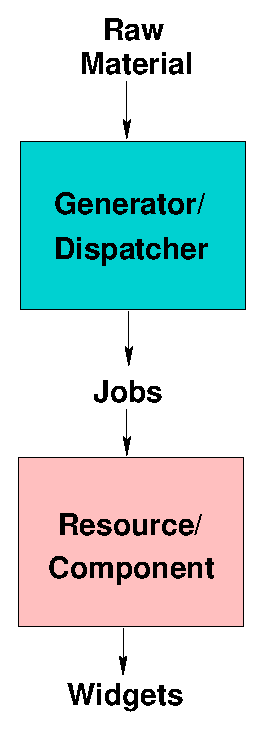
\includegraphics[width=1in]{oldsys}
\hskip1in
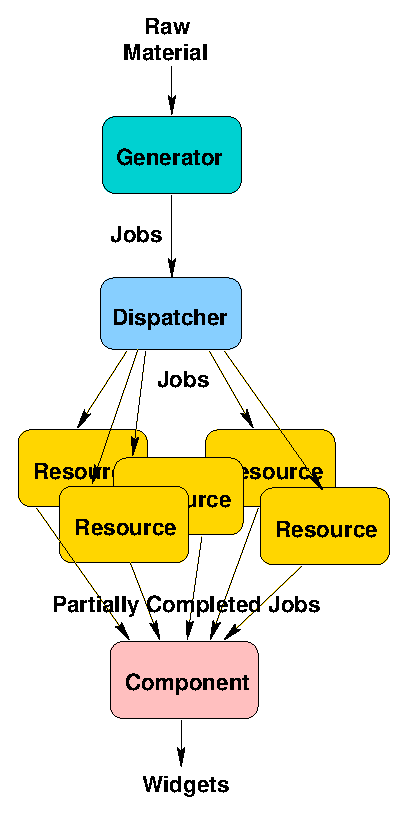
\includegraphics[width=2in]{newsys}\\
\end{center}
\hskip1.7in(a)\hskip2.2in(b)\\
\caption{(a) Model of original industrial process system; (b) Model of
new proposed system.}
\label{fig:ipsys}
\end{figure}

The new system consists of:

\begin{enumerate}
\item A Generator unit that generates jobs in much the
same way as the original.  It passes the job to:
\item A Dispatcher unit, which dispatches the jobs to one or more
Resource units.  The Dispatcher also handles requests from idle
Resource units for more jobs.  
\item The Resource units perform phase 1 of the process and can then
check to see if the job has errors.  The job is thus either discarded
at this point, or passed on to a single Component unit.
\item The Component unit performs the second phase of the process to
complete the job and create the resulting widget.
\end{enumerate}

The new system improves upon the old in many ways.  The new machines are more
energy efficient -- a system consisting of one of each unit type uses less
power than the old system.  Adding more Resource units increases the power
usage of course.  The new machine also allows for several jobs to be
undergoing phase 1 -- the long phase simultaneously, in addition to pipelining
phase 1 and phase 2.  Further, it eliminates the processing of junk jobs in
phase 2 by detecting them immediately after phase 1.  In addition, maintenance
costs are lower, and breakdowns are predicted to occur on a resource once per
20000 jobs processed, with a breakdown time of three hours.  

It does however require more supervision: 2 workers are need to
operate the Component unit, and one for each other type of unit. Old
and new units still take the same time to process jobs: a random value
between 1 and 10 times the job complexity for the first phase and a
random value between 1 and 3 times the job complexity for the second
phase. And finally, the new system is much more expensive to purchase.

\begin{verbatim}
PURCHASE COSTS:
Generator:  $1500 
Dispatcher: $2500
Resource:   $3750
Component:  $2795

POWER COSTS per 8 hours operation:
Generator:  $ 30 
Dispatcher: $ 30
Resource:   $ 45
Component:  $ 15
\end{verbatim}

Thus, the company board wants to know several things:

\begin{enumerate}
\item How long does it take for the old system to pay for itself?
\item And the new?  Want to try this with various numbers of Resource units.
\item What number of resource units produces the max profit?
\item What number of resource units pays for itself the fastest?
\end{enumerate}

Because of the parallelism at phase 1, complex jobs might tie up resources,
but simpler ones might still pass through and keep the Component unit
busy. Thus it is hard to predict how much this system will improve over the
old, and with the addition of Resource units.  Thus we should strive to see
how to make the idle time of the Component close to zero with the fewest
resources. 

\subsection{Modelling the Original System}

Although we could compute the performance of the original system from
the available data, it would help us get started if we just simulate
the original system.  We can compare our results to what is actually
happening to verify its correctness.

There are exactly 2 entities in the old system, the Generator/Dispatcher and
the Resource/Component.  To simulate this, we must create a POSE module (we'll
call this one the 'oldsys'), consisting of a .ci, a .h and a .C file.  These
files differ in syntax slightly from the equivalent Charm++ code files.

\subsubsection{The Interface File}

A POSE module is made up of a Charm++ Interface file ({\tt .ci}), a
header file ({\tt .h}) containing message and class declarations, and
an implementation file ({\tt .C}).  Here's the interface for the old
system, {\tt oldsys.ci}:

\begin{verbatim}
message Job;
message Stats;

poser GeneratorDispatcher : sim opt chpt {
  entry GeneratorDispatcher(eventMsg *);
  // Event methods
  entry [event] void receive(Job *);
};

poser ResourceComponent : sim opt chpt {
  entry ResourceComponent(eventMsg *);
  // Event methods
  entry [event] void receive(Job *);
  entry [event] void processJob(eventMsg *);
  // Non-Event Entry methods
  entry [sync] Stats *getStats(void);
};
\end{verbatim}

Note that we do not use the Charm++ module syntax.  We do however declare our
messages, and then the objects.  Note that simulation objects are called
'posers' rather than 'chares', and that a poser behaves as a chare for the
most part.  It is actually implemented as a chare array element, but this
should be mostly invisible to the user.  

After the colon in the poser declaration, we have three special terms that
designate the simulation behavior and representation of the object.  The first
term is for the wrapper behavior.  The wrapper will control all access to the
object.  Currently, there is only one wrapper class, sim, and all future
wrapper classes should inherit from sim.  Second, we have the simulation
strategy.  This determines the simulation behavior of the object.  Currently,
we have two basic strategies, con (for conservative) and opt (for optimistic)
which control the synchronization of the incoming timestamped events.  The
focus of POSE is to eke out performance improvements using the optimistic
synchronization mechanism, so we'll select opt for this example.  The final
term designates the state representation for the object, i.e. it provides a
policy by which the state can be updated, saved and rolled back.  It also
maintains a special object virtual time (ovt) for each object.  There is a
basic representation, rep, which only provides the ovt mechanism, and and more
complex chpt, which allows, for checkpointing and state recovery.  In general,
we only need rep to accompany the con strategy, but if we are using opt, we
will need checkpointing and state recovery, so we will use chpt here. 

The constructor should be considered a timestamped event.  In addition, entry
methods are designated at timestamped events by the 'event' tag.  Events
*must* pass a message.  If no data is passed, and the method would otherwise
be void, the message type should be eventMsg *.  This is because we need to
put a timestamp on messages and the eventMsg type corresponds to a timestamped
void message. 

\subsubsection{The Header File}

Now we examine the header file for the old system model,
{\tt oldsys.h}.  First we define the messages we will be using:

\begin{verbatim}
class Stats : public CMessage_Stats {
 public:
  int junkJobs, completedJobs, idleTime;
};
\end{verbatim}

Stats is an ordinary Charm++ message.  Job, however, is a POSE event message.
This means that we leave out the \verb|: public CMessage_Job| bit and provide
operator= and pup methods, and treat Job as if it were derived from eventMsg.
Note also that Job has a "next" field which will allow us to store these Job
messages in a queue.

\begin{verbatim}
class Job {
 public:
  int complexity, id;
  Job *next;
  Job& operator=(const Job& obj) {
    eventMsg::operator=(obj);
    complexity = obj.complexity;
    id = obj.id;
    return *this;
  }
  void pup(PUP::er &p) {
    eventMsg::pup(p);
    p(complexity); p(id);
  }
};
\end{verbatim}

Next we define the poser chares:

\begin{verbatim}
class GeneratorDispatcher {
 public:
  GeneratorDispatcher() { }
  GeneratorDispatcher(eventMsg *);
  ~GeneratorDispatcher() { }
  void pup(PUP::er &p) {
    chpt<state_GeneratorDispatcher>::pup(p);
  }
  GeneratorDispatcher& operator=(const GeneratorDispatcher& obj) {
    rep::operator=(obj);
    return *this;
  }  
  // Event methods
  void receive(Job *);
  void receive_anti(Job *) { restore(this); }
  void receive_commit(Job *) { }
};
\end{verbatim}

Note that a parameterless contructor, a destructor, a pup, and an
operator= are all required for a poser.  Also, for each event method,
a commit method is required.  Further, for each event method of a
class that uses the optimistic synchronization strategy, an anti
method is required as well.  After the receive event method is called,
the \verb|receive_anti| method simply makes use of the checkpointing
that is happening to restore the state of the object prior to the
receive call.

Note also the difference in the superclass pup and assignment
operators.  The class you are defining will actually be a subclass of
the representation component in POSE.  Since we've chosen a
checkpointing representation, we use the chpt parent pup to pack up or
unpack the entire checkpointed state of the object (pups are used for
migration -- see the Charm++ manual).  The assignment operator
in POSE is used for actually copying the state of the object during
checkpointing.  Thus you only copy the immediate state, and not all the
checkpointed information, so in this case you only need to call the
assignment of the base class rep, which assures that the ovt is copied
properly. 

\begin{verbatim}
class ResourceComponent {
  int myHandle, junkJobs, completedJobs;
  int idleTime, idle, idleStart;
  Job *queue, *tail;
 public:
  ResourceComponent() { 
    junkJobs = completedJobs = idleTime = idle = idleStart = 0; 
  }
  ResourceComponent(eventMsg *);
  ~ResourceComponent() { 
    Job *tmp = queue;
    while (tmp) {
      queue = tmp->next;
      delete(tmp);
      tmp = queue;
    }
  }
  void pup(PUP::er &p) {
    Job *tmp;
    int count, i;
    chpt<state_ResourceComponent>::pup(p);
    p(myHandle); p(junkJobs); p(completedJobs); 
    p(idleTime); p(idle); p(idleStart);

    if (p.isUnpacking()) {
      p(count);
      queue = tail = NULL;
      if (count > 0)
        tmp = queue = new Job;
      for (i=0; i<count; i++) {
        tmp->pup(p);
        tmp->next = NULL;
        if (i+1 < count) {
          tmp->next = new Job;
          tmp = tmp->next;
        }
        if (i+1 == count) tail = tmp;
      }
    }
    else {
      count = 0;
      tmp = queue;
      while (tmp) {
        count++;
        tmp = tmp->next;
      }
      p(count);
      tmp = queue;
      while (tmp) {
        tmp->pup(p);
        tmp = tmp->next;
      }
    }      
  }
  ResourceComponent& operator=(const ResourceComponent& obj) {
    Job *tmp1, *tmp2;
    rep::operator=(obj);
    myHandle = obj.myHandle;
    junkJobs = obj.junkJobs;
    completedJobs = obj.completedJobs;
    idleTime = obj.idleTime;
    idle = obj.idle;
    idleStart = obj.idleStart;
    queue = tail = NULL;
    tmp1 = obj.queue;
    if (tmp1) {
      tmp2 = queue = tail = new Job;
      tmp2->next = NULL;
    }
    while (tmp1) {
      (*tmp2) = (*tmp1);
      if (tmp1->next) {
        tmp2->next = new Job;
        tmp2 = tmp2->next;
        tail = tmp2;
        tmp2->next = NULL;
      }
      tmp1 = tmp1->next;
    }
    return *this;
  }  
  // Event methods
  void receive(Job *);
  void receive_anti(Job *) { restore(this); }
  void receive_commit(Job *) { }
  void processJob(eventMsg *);
  void processJob_anti(eventMsg *) { restore(this); }
  void processJob_commit(eventMsg *) { }
  // Non-Event Entry methods
  Stats *getStats();
};
\end{verbatim}

Note that non-event entry methods are still possible and work like regular
entry methods in Charm++.  The above example uses a sync method to send data
to the main chare at the end of the program.  Note that commit methods are
typically empty.  The user may wish to use commit methods to perform special
actions when an event has been committed to (print statistics, debugging, or
other information), however, the state of the object when an event is
committed may differ from when the event was actually executed, so this should
be used with caution, especially where modifications to the state are
concerned.  

\subsubsection{The Implementation File}

Finally, we look at the Implementation of our POSE module,
{\tt oldsys.C} and see how a POSE simulation fits together: 

\begin{verbatim}
GeneratorDispatcher::GeneratorDispatcher(eventMsg *m)
{
  init(m);
  Job *j = new Job;
  int i;

  delete(m);
  eventMsg *e = new eventMsg;
  POSE_create(ResourceComponent(e), 1, 0);

  j->complexity = (lrand48() % 10) + 1;
  j->id = 0;
  POSE_invoke(receive(j), GeneratorDispatcher, 0, 0);
  initComplete();
}
\end{verbatim}

Primary constructors for posers must have a call to init with the incoming
message as parameter.  Constructor messages must be deleted when you are done
with them.  This does not hold for event methods -- one should NOT delete
event messages sent to event methods.  After the data fields of the object are
initialized, initComplete must be called.  This call could go anywhere after
all initializations are complete, or be placed at the end of the constructor
for simplicity. 

Inside a POSE module, we can create other posers using the \verb|POSE_create|
function.  To invoke event methods on an object, we use some form of the
\verb|POSE_invoke| function.  The other forms this may take are
\verb|POSE_invoke_at| and
\verb|POSE_local_invoke|.  

\begin{verbatim}
void GeneratorDispatcher::receive(Job *j) { Job *newJ1, *newJ2;

  checkpoint(this);
  update(j->timestamp);
  if (j->timestamp < 28800 - 1) {
    newJ1 = new Job;
    newJ1->complexity = (lrand48() % 10) + 1;
    newJ1->id = (j->timestamp)+1;
    POSE_local_invoke(receive(newJ1), 1);
  }
  newJ2 = new Job;
  newJ2->complexity = j->complexity;
  newJ2->id = j->id;
  POSE_invoke(receive(newJ2), ResourceComponent, 1, 0);
}
\end{verbatim}

In event methods, we must call a few functions before any other activity.  One
is the update function, which takes the incoming message and adjusts local
time (ovt) accordingly.  The other function is used only when we are
checkpointing, and it checkpoints the state of the object before we make any
changes to it.  Thus is is necessary to call both these functions before any
state changes are made and before any time elapses in the method. 

\begin{verbatim}
ResourceComponent::ResourceComponent(eventMsg *m)
{
  init(m);
  myHandle = 1;
  idle = 1;
  junkJobs = completedJobs = 0;
  idleTime = 0;
  queue = tail = NULL;
  delete m;
  initComplete();
}

void ResourceComponent::receive(Job *j)
{
  eventMsg *m1;
  Job *tmp = new Job;

  checkpoint(this);
  update(j->timestamp);
  
  if (!tail) {
    tail = queue = tmp;
    tmp->next = NULL;
  }
  else {
    tail->next = tmp;
    tmp->next = NULL;
    tail = tmp;
  }

  tmp->complexity = j->complexity;
  tmp->id = j->id;
  
  if (idle) {
    idleTime += ovt - idleStart;
    idle = 0;
    m1 = new eventMsg;
    POSE_local_invoke(processJob(m1), 0);
  }
}

void ResourceComponent::processJob(eventMsg *m)
{
  Job *j = queue;
  eventMsg *m1;

  checkpoint(this);
  update(m->timestamp);
  if (!queue) {
    CkPrintf("ERROR: no jobs in queue.\n");
    return;
  }
  queue = queue->next;
  if (!queue) tail = NULL;

  // Phase 1
  elapse(((lrand48() % 10) + 1) * j->complexity);

  // Phase 2
  elapse(((lrand48() % 3) + 1) * j->complexity);

  if (lrand48() % 100 > 97)
    junkJobs++;
  else
    completedJobs++;
  if (!queue) {
    idle = 1;
    idleStart = ovt;
  }
  else {
    m1 = new eventMsg;
    POSE_local_invoke(processJob(m1), 0);
  }
}
\end{verbatim}

The above method illustrates one of the ways to specify the passage of
simulation time.  The other way is to specify an offset when invoking events
on posers.

\begin{verbatim}
Stats *ResourceComponent::getStats()
{
  Stats *m1 = new Stats;

  m1->junkJobs = junkJobs;
  m1->completedJobs = completedJobs;
  m1->idleTime = idleTime;
  return m1;
}
\end{verbatim}

Note that each poser has an id associated with it.  In the above example,
since there are only two objects, it is hardly noticeable, but the
GeneratorDispatcher has an id of 0, and the ResourceComponent has an id of 1.
These ids are the means by which we refer to all the posers in a system.
Their usage should be apparent in the reference section of this manual. 


\subsubsection{The Main Program}

How does one make use of a POSE module?  We show how the POSE
environment is set up in the following code samples, but first, we
need to discuss how to process the {\tt oldsys} module so it is
usable by Charm++. To do this, there exists a perl script {\tt
etrans.pl}.  We pass in the POSE module name and the script translates
the POSE module into Charm++ code.

\begin{verbatim}
> etrans.pl oldsys
[processing info]
>
\end{verbatim}

This translator will attempt to alert you if you've done something
obviously wrong with relation to POSE, but it will not pick up Charm++
or C++ syntax errors.  It will generate three new files: files {\tt
X[.ci$|$.h$|$.C]} will be translated to {\tt X\_sim[.ci$|$.h$|$.C]}.  These
new files are what you use to build the executable simulation.

Now let's build a simple main module that starts up a POSE simulation
on the module {\tt oldsys} and then gathers statistics, prints them
and exits.

Here's the {\tt pgm.ci} file:

\begin{verbatim}
mainmodule Pgm {
  extern module oldsys;
  readonly CkChareID mainhandle;
  
  mainchare main {
    entry main();
    entry void wrapUp();
  };
};
\end{verbatim}

This is a simple Charm++ program that includes the {\tt oldsys}
module.  Now for the {\tt pgm.h} file:

\begin{verbatim}
#include "Pgm.decl.h"

CkChareID mainhandle;

class main : public Chare {
public:
  main(CkArgMsg *m);
  main(CkMigrateMessage *) {};
  void wrapUp();
};
\end{verbatim}

Nothing new here if you know Charm++.  We desire that the {\tt wrapUp}
method gets called at the end of the program and requests statistics
from the ResourceComponent unit and prints them and exits.  We'll see
how this is done shortly.  Finally, we have the main program, {\tt
pgm.C}:

\begin{verbatim}
#include "pgm.h"
#include "Pgm.def.h"
#include "pose.h"
#include "oldsys_sim.h"

main::main(CkArgMsg *m)
{ 
  CkGetChareID(&mainhandle);
  CProxy_main M(mainhandle);

  srand48(42);

  POSE_endtime = 28800;
  POSE_init();
  POSE_registerCallBack(CkCallback(CkIndex_main::wrapUp(), M));

  eventMsg *e = new eventMsg;
  (*(CProxy_GeneratorDispatcher *) & POSE_Objects)[0].insert(e);

  POSE_start();
}

void main::wrapUp()
{
  CkPrintf("And now for something completely different...\n");
  Stats *results;

  results = (*(CProxy_ResourceComponent *) & POSE_Objects)[1].getStats();
  CkPrintf("# completed jobs = %d; # junk jobs = %d; idle time = %d\n", 
	   results->completedJobs, results->junkJobs, results->idleTime);  
  CkExit();
}
\end{verbatim}

There are several things of note here. First, we include both {\tt
pose.h} and {\tt oldsys\_sim.h} here.  Second, we set a variable called
{\tt POSE\_endtime}.  This variable specifies to POSE what time (in
simulation time units) to stop at.  For this particular example, our
time units are seconds, and we want the simulation to run for an
eight-hour work shift.  If this variable is not set, the simulation
runs until quiescence is detected.

The next thing we do is initialize the POSE environment.  Fourth, we
register {\tt wrapUp} as a callback, so that when the simulation is
completed, we can print out the information we are interested in.  

Next, we create the GeneratorDispatcher (which in turn creates the
ResourceComponent).  This ugly syntax is currently necessary for
making calls into POSE from outside of POSE modules.  It will be
replaced soon with similar calls as used inside a POSE module.  Now
that the environment is set up, we start the simulation with a call to
{\tt POSE\_start}.  The {\tt wrapUp} method also contains an ugly
syntax line, and a replacement for this is also in the works.

\subsection{Modelling the New System}

For the new system, we want to separate the Generator from the
Dispatcher, and the Resource from the Component, and make the number
of resources a parameter to the simulation.  The code for this new
version is available in the appendix.  

One interesting run of this program with a single resource reveals the
improvement in the new system allowed by the fact that the two phases
of the Resource and the Component can now be pipelined to overlap.
This results in many more completed jobs, but note that the Component
is still idle for over five hours of the eight-hour work day!

\begin{verbatim}
Resource 1: # junk jobs = 15;        idle time = 36
Component:  # completed jobs = 936;  idle time = 18501
\end{verbatim}

Adding more resources reduces this idle time and dramatically improves
the system output.  Here is the result for four resources:

\begin{verbatim}
Resource 1: # junk jobs = 22;         idle time = 36
Resource 2: # junk jobs = 17;         idle time = 141
Resource 3: # junk jobs = 23;         idle time = 60
Resource 4: # junk jobs = 19;         idle time = 55
Component:  # completed jobs = 3702;  idle time = 36
\end{verbatim}

A final, very interesting thing to note:  because of the randomness
applied to processing jobs of various complexities, adding more
resources to this system still improves the number of completed jobs,
{\it even though the idle time above is only 36 seconds!}  This is
because less complex jobs filter through the larger system faster.
These results can be viewed below.  We used eight resources in this
run.

\begin{verbatim}
Resource 1: # junk jobs = 24;        idle time = 36
Resource 2: # junk jobs = 17;        idle time = 14
Resource 3: # junk jobs = 18;        idle time = 60
Resource 4: # junk jobs = 25;        idle time = 55
Resource 5: # junk jobs = 20;        idle time = 38
Resource 6: # junk jobs = 21;        idle time = 79
Resource 7: # junk jobs = 15;        idle time = 243
Resource 8: # junk jobs = 15;        idle time = 74
Component:  # completed jobs = 7509; idle time = 13
\end{verbatim}

Thus we see how simulation can illustrate unpredictable behaviors in a
system.  For more details on the Industrial Process Simulator, see the
enhanced code for the original system, the code for the new system,
and an analysis of the results, in the appendix of this manual.

\section{Programmer's Reference}

This section details syntax and usage of POSE constructs.  The last
subsection lists all constructs and their usage in brief.

\subsection{POSE Modules}

A POSE module is similar to a Charm++ module.  It is comprised of 
{\tt .ci}, {\tt .h}, and {\tt .C} files.  Several posers can be
described in one module, and the module can include regular chares as
well.  The module is translated into Charm++ before the simulation can
be compiled.  This translation generates files suffixed {\tt \_sim.ci},
{\tt \_sim.h}, and {\tt \_sim.C}.  

\subsection{Event Message and Poser Interface Description}

Messages, be they event messages or otherwise, are described in the
{\tt .ci} file exactly the way they are in Charm++, with the exception
that parameter marshalling cannot be used, and thus you must declare
them in the {\tt .h} file.  

~\\
\noindent{\tt {\bf message} {\it myMessage};}\\

Posers are described similar to chares, with a few exceptions.  First,
the {\tt poser} keyword is used to denote that the class is a POSE
simulation object class.  Second, event methods are tagged with the
keyword {\tt event} in square brackets. Finally, three components are
specified which indicate how objects of the poser class are to be
simulated.  The {\it sim} component controls the wrapper class and
event queue used by the object (see section ? for more on the internal
representation of a poser).  The {\it strat} component controls the
synchronization strategy the object should use ({\it optimistic} or
{\it conservative}).  The {\it rep} component specifies the global
state representation, which controls how the global state is kept
accurate depending on the synchronization strategy being used.

~\\
\noindent{\tt {\bf poser} {\it mySim} : {\it sim strat rep} \{\\
\indent {\bf entry} {\it mySim}({\it myMessage} *);\\
\indent {\bf entry} [{\bf event}] void {\it myEventMethod}({\bf eventMsg} *);\\
\indent ...\\
\noindent \};}\\

Note that the constructors and event methods of a poser must take an
event message as parameter.  If there is no data that needs to be
passed in to the method, then the parameter should be of type {\tt
eventMsg *}.  This ensures that the POSE system will be able to
timestamp the event.

\subsection{Declaring Event Messages and Posers}

Event messages are declared with no reference to what they might
inherit from (unlike in Charm++).  In addition, they must have {\tt
operator=} defined for them.

~\\
\noindent{\tt class {\it myMessage} \{\\
\indent  public:\\
\indent   int someData;\\
\indent   {\it myMessage}\& operator=(const {\it myMessage}\& obj) \{\\
\indent\indent     {\bf eventMsg}::operator=(obj);\\
\indent\indent     someData = obj.someData;\\
\indent\indent     return *this;\\
\indent   \}\\
\noindent \};}\\

Similarly, posers do not refer to a base class when they are
declared.  Posers are required to have a void constructor declared
that simply initializes the data to sensible values.  A destructor
must be provided as well.  In addition, a {\tt pup} and {\tt
operator=} must be provided.  The {\tt pup} method should call the
{\tt pup} method of the global state representation class being used.

~\\
\noindent{\tt class {\it mySim} \{\\
\indent int anInt; float aFloat; char aString[20];
\indent public:\\
\indent {\it mySim}();\\
\indent {\it mySim}({\it myMessage} *m);\\
\indent \verb|~|{\it mySim}();\\
\indent void pup(PUP::er \&p);\\
\indent {\it mySim}\& operator=(const {\it mySim}\& obj);\\
\indent void {\it myEventMethod}({\bf eventMsg} *m);\\
\indent void {\it myEventMethod}{\bf \_anti}({\bf eventMsg} *m);\\
\indent void {\it myEventMethod}{\bf \_commit}({\bf eventMsg} *m);\\
\indent ...\\
\noindent \};}\\

Further, for each event method, a commit method should be declared,
and if the synchronization strategy being used is optimistic or
involves any sort of rollback, an anti-method should also be provided.
The syntax of these declarations is shown above.  Their usage and
implementation will be described next.

\subsection{Implementing Posers}

The void constructor for a poser should be defined however the user
sees fit.  It could be given an empty body and should still work for
POSE.  The entry method constructors (those described in the {\tt .ci}
file should follow the template below:

~\\
\noindent{\tt {\it mySim}::{\it mySim}({\it myMessage} *m)\\
\noindent\{\\
\indent {\bf init}(m);\\
\indent // initializations from $m$\\
\indent ...\\
\indent delete m;\\
\indent ...\\
\indent {\bf initComplete}();\\
\noindent \};}\\

The {\tt init} function adjust the objects OVT to the correct start
point, while the {\tt initComplete} function allows the object to
start processing incoming events.  Note that while the incoming
message m may be deleted here in the constructor, event messages sent
to event methods should {\bf not} be deleted.

An event method should have the following form:

~\\
\noindent{\tt void {\it mySim}::{\it myEventMethod}(eventMsg *m) \{\\
\indent {\bf checkpoint}(this);\\
\indent {\bf update}(m->timestamp);\\
\indent // body of method \\
\noindent \};}\\

All event methods should make the call to {\tt update} and pass in the
timestamp of the incoming message.  This synchronizes the object's OVT
with the timestamp of the event.  Also, if the object uses
checkpointing for its global state representation, you will need to
checkpoint the current state of the object as shown above.

\subsection{Creation of Poser Objects}

Posers are created within a module using the following syntax:

~\\
\noindent {\tt int hdl = 13;\\
\noindent {\it myMessage} *m = new {\it myMessage};\\
\noindent m->someData = 34;\\
\noindent {\bf POSE\_create}({\it mySim}(m), hdl, 0);}\\

This creates a {\tt mySim} object that comes into existence at
simulation time zero, and can be referred to by the handle 13.  

Creating a poser from outside the module is somewhat more complex:

~\\
\noindent {\tt int hdl = 13;\\
\noindent {\it myMessage} *m = new {\it myMessage};\\
\noindent m->someData = 34;\\
\noindent m->{\bf Timestamp}(0);\\
\noindent (*(CProxy\_{\it mySim} *) \& {\bf POSE\_Objects})[hdl].insert(m);}\\

This is similar to what the module code ultimately gets translated to,
and should be replaced by a macro with similar syntax soon.

\subsection{Event Method Invocations}

Event method invocations vary significantly from entry method
invocations in Charm++, and various forms should be used depending on
where the event method is being invoked.  In addition, event messages
sent to an event method should be allocated specifically for an event
invocation, and cannot be recycled or deleted.

There are three ways to send events within a POSE module.  The first
and most commonly used way involves specifying and offset in
simulation time from the current time.  The syntax follows:

~\\
\noindent {\tt aMsg = new {\bf eventMsg};\\
\noindent {\bf POSE\_invoke}({\it myEventMethod}(aMsg), {\it
mySim}, hdl, 0);}\\

Here, we've created an {\tt eventMsg} and sent it to {\tt
myEventMethod}, an event entry point on {\tt mySim}.  {\tt mySim} was
created at handle {\tt hdl}, and we want the event to take place now,
i.e. at the current simulation time, so the offset is zero.  

The second way to send an event is reserved for use by non-poser
objects within the module.  It should not be used by posers.  This
version allows you to specify an absolute simulation time at which the
event happens (as opposed to an offset to the current time).  Since
non-poser objects are not a part of the simulation, they do not have a
current time, or OVT, by which to specify an offset.  The syntax is
nearly identical to that above, only the last parameter is an absolute
time.

~\\
\noindent {\tt aMsg = new {\bf eventMsg};\\
\noindent {\bf POSE\_invoke\_at}({\it myEventMethod}(aMsg), {\it
mySim}, hdl, 56);}\\

Posers should not use this approach because of the risk of specifying
an absolute time that is earlier than the current time on the object
sending the event.  

The third approach is useful when an object send events to itself.  It
is simply a slightly shorter syntax for the same thing as {\tt
POSE\_invoke}: 

~\\
\noindent {\tt aMsg = new {\bf eventMsg};\\
\noindent {\bf POSE\_local\_invoke}({\it myEventMethod}(aMsg), offset);}\\

Event methods can be injected into the system from outside the module,
but this is not recommended.  

\subsection{Elapsing Simulation Time}

We've seen in the previous section how it is possible to advance
simulation time by generating events with non-zero offsets of current
time.  When such events are received on an object, if the object is
behind, it brings itself in sync with the event by calling the {\tt
update} function with the incoming event message.  

It is also possible to elapse time on an object while the object is
executing an event.  This is accomplished thus:

~\\
\noindent {\tt {\bf elapse}(42);}\\

The example above would simulate the passage of forty-two time units
by adding as much to the object's current OVT.

\subsection{Interacting with a POSE Module and the POSE System}

{\it Discuss how to interface main program with POSE module; discuss
initialization of POSE, etc.}

\subsection{Glossary of POSE-specific Terms}

\begin{itemize}
\item {\tt void {\bf POSE\_init}()}\\
	$\circ$ Initializes various items in POSE; creates the load balancer
	if load balancing is turned on; initializes the statistics
	gathering facility if statistics are turned on.\\
	$\circ$ Must be called in user's main program prior to creation of any
	simulation objects or reference to any other POSE construct.
\item {\tt void {\bf POSE\_start}()}\\
	$\circ$ Sets busy wait to default if none specified; starts
	quiescence detection; starts simulation timer.\\
	$\circ$ Must be called in user's main program when simulation
	should start.
\item {\tt void {\bf POSE\_registerCallBack}(CkCallback cb)}\\
	$\circ$ Registers callback function with POSE -- when program
	ends or quiesces, function is called.\\
	$\circ$ CkCallback is created with the index of the callback
	function and a proxy to the object that function is to be
	called on.  For example, to register the function {\tt wrapUp}
	in the main module as a callback:

\begin{verbatim}
  CProxy_main M(mainhandle);
  POSE_registerCallBack(CkCallback(CkIndex_main::wrapUp(), M));
\end{verbatim}

\item {\tt void {\bf POSE\_stop}()}\\
	$\circ$ Commits remaining events; prints final time and
	statistics (if on); calls callback function.\\
	$\circ$ Called internally when quiescence is detected or
	program reaches {\tt POSE\_endtime}.
\item {\tt void {\bf POSE\_exit}()}\\
	$\circ$ Similar to {\tt CkExit()}.
\item {\tt void {\bf POSE\_set\_busy\_wait}(int n)}\\
	$\circ$ Used to control granularity of events; when calling
	{\tt POSE\_busy\_wait}, program busywaits for time to compute $fib(n)$.
\item {\tt void {\bf POSE\_busy\_wait}()}\\
	$\circ$ Busywait for time to compute $fib(n)$ where n is either
	1 or set by {\tt POSE\_set\_busy\_wait}.
\item {\tt {\bf POSE\_endtime}}\\
	$\circ$ Set this to $n$ and program will terminate when global
	virtual time (GVT) reaches $n$.
\item {\tt void {\bf POSE\_create}({\it constructorName}(eventMsg *m), int
handle, int atTime)}\\
	$\circ$ Creates a poser object given its constructor, an event
	message $m$ of the appropriate type, any integer as the handle
	(by which the object will be referred from then on), and a
	time (in simulation timesteps) at which it should be created.\\ 
	$\circ$ The handle can be thought of as a chare array element
	index in Charm++.
\item {\tt void {\bf POSE\_invoke\_at}({\it methodName}(eventMsg *m),
{\it className}, int handle, int atTime)}\\
	$\circ$ Send a {\it methodName} event with message $m$ to an
	object of type {\it className} designated by handle $handle$
	at time specified by $atTime$.\\
	$\circ$ This can be used by non-poser objects in the POSE
	module to inject events into the system being simulated.  It
	should not be used by a poser object to generate an event.
\item {\tt void {\bf POSE\_invoke}({\it methodName}(eventMsg *m),
{\it className}, int handle, int timeOffset)}\\
	$\circ$ Send a {\it methodName} event with message $m$ to an
	object of type {\it className} designated by handle $handle$
	at current OVT + $timeOffset$.\\
	$\circ$ This is used by poser objects to send events from one
	poser to another.
\item {\tt void {\bf POSE\_local\_invoke}({\it methodName}(eventMsg
	*m), int timeOffset)}\\
	$\circ$ Send a {\it methodName} event with message $m$ to this
	object at current OVT + $timeOffset$.\\
	$\circ$ This is used by poser objects to send events to themselves.
\item {\tt void {\bf init}(eventMsg *m)}\\
	$\circ$ Initializes representation-specific data fields (such
	as OVT and links to other components of the poser).
\item {\tt void {\bf initComplete}()}\\
	$\circ$ Tells the POSE system that the object is ready to
	start processing events.
\item {\tt void {\bf checkpoint}(rep *t)}\\
	$\circ$ Checkpoints the current state, according to
	checkpointing frequency.
\item {\tt void {\bf restore}(rep *t)}\\
	$\circ$ Restores the state from checkpointed data.
\item {\tt void {\bf update}(eventMsg *m)}\\
	$\circ$ Brings OVT into sync with event timestamp: if OVT <
	timestamp, OVT is set to timestamp.
\item {\tt void {\bf CommitPrint}(char *s)}\\
	$\circ$ Buffered print statement; prints when event is
	committed.\\
	$\circ$ Currently, must be called on the wrapper class
	(parent) to work properly, but a fix for this is in the works.
\item {\tt void {\bf elapse}(int n)}\\
	$\circ$ Elapse $n$ simulation time units.
\item {\tt {\bf poser}}\\
	$\circ$ Keyword (used in place of chare) to denote a poser
	object in the {\tt .ci} file of a POSE module.
\item {\tt {\bf event}}\\
	$\circ$ Keyword used in square brackets in the {\tt .ci} file
	of a POSE module to denote that the entry method is an event method.
\item {\tt {\bf eventMsg}}\\
	$\circ$ Base class for all event messages; provides timestamp,
	priority and many other properties.
\item {\tt {\bf sim}}\\
	$\circ$ Base class of all wrapper classes.
\item {\tt {\bf strat}}\\
	$\circ$ Base class of all strategy classes.
\item {\tt {\bf con}}\\
	$\circ$ Simple conservative strategy class.
\item {\tt {\bf opt}}\\
	$\circ$ Simple optimistic strategy class.
\item {\tt {\bf rep}}\\
	$\circ$ Base class for all representation classes.
\item {\tt {\bf chpt}}\\
	$\circ$ Simple checkpointing representation class.
\item {\tt {\bf ovt}}\\
	$\circ$ Accessible data field of the {\tt rep} class; denotes
	the object virtual time (OVT) of the object; avoid using
	directly, may become private in the future.
\end{itemize}


\begin{figure}[h]
\begin{center}
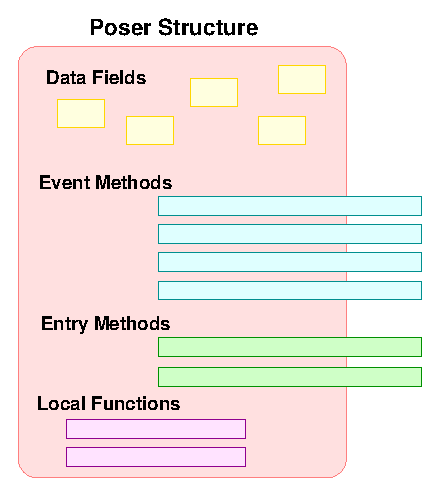
\includegraphics[width=1.5in]{base_struct}
\end{center}
\caption{The user's view of a {\it poser}, or simulation object, in POSE.}
\label{fig:base_struct}
\end{figure}

\section{Delving Deeper into POSE}

This section describes some of the internal representations used by
POSE, and how to write more efficient parallel discrete event
simulations.  The first part deals with how POSE simulation objects, or
{\it posers}, are represented in POSE.  It is useful to know a little
about this internal representation, when deciding what sort of
sychronization strategy and global state representation to use.  It is
also essential to know this structure if you want to add new
strategies and representations.  Even the simulation wrapper class
(described below) could be subclassed, to modify how the event queue
gets handled. 

\begin{figure}[h]
\begin{center}
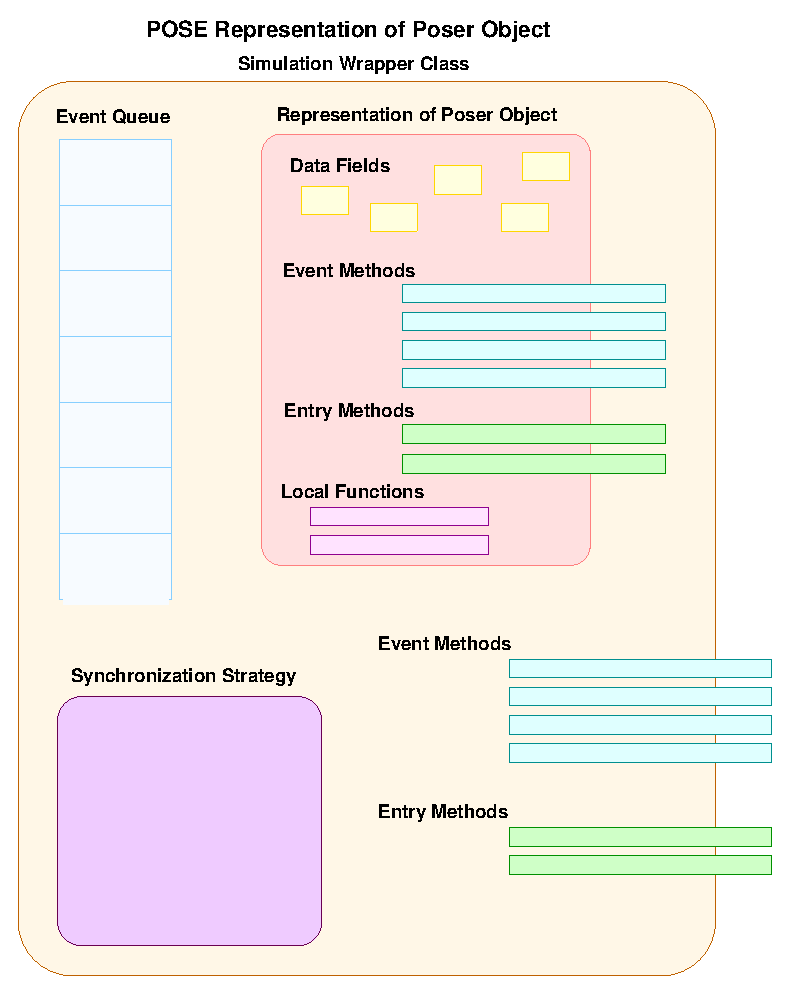
\includegraphics[width=2.5in]{pose_struct}
\hskip0.5in
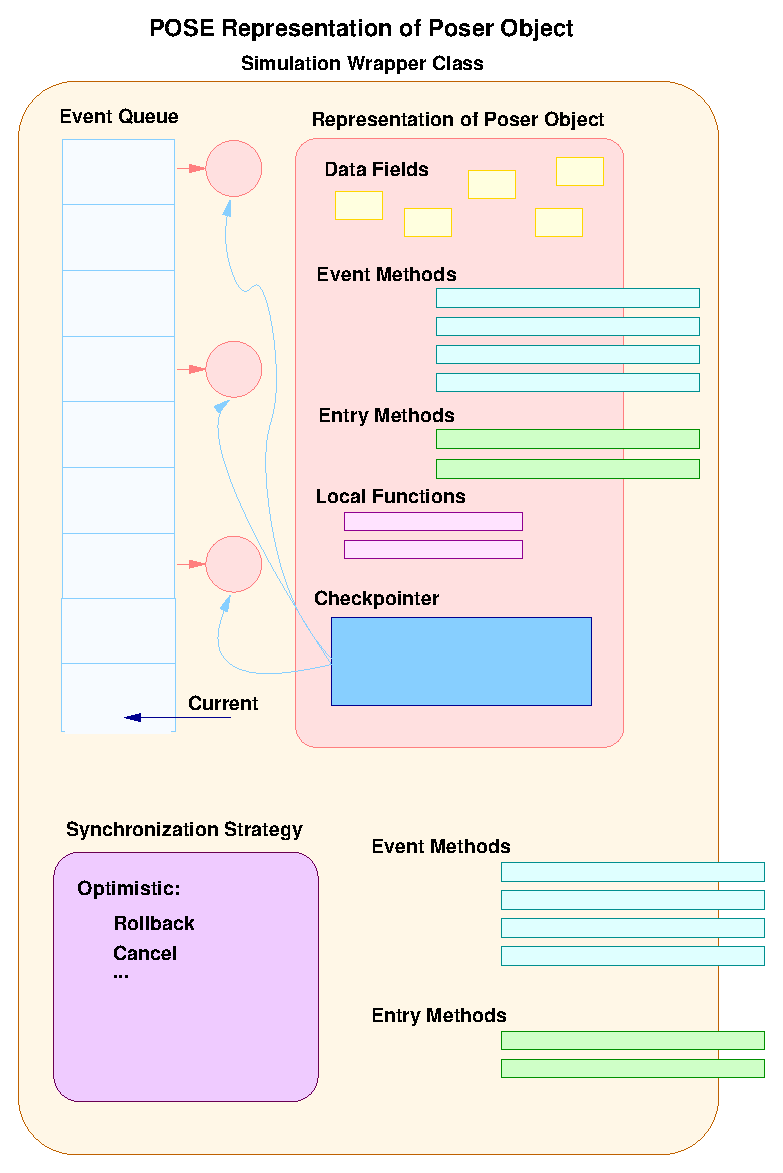
\includegraphics[width=2.5in]{opt_struct}
\end{center}
\hskip1.7in(a)\hskip2.2in(b)\\
\caption{(a) Internal representation of a {\it poser}; (b) internal representation of a {\it poser} using optimistic
synchronization and checkpointing.}
\label{fig:pose_struct}
\end{figure}

\subsection{Structure}

The user of POSE expresses a simulation object that looks very similar
to a C++ or Charm++ object.  This poser has data fields that make up a
part of the simulations global state, and events, which look nearly
identical to Charm++ entry methods.  Further, it can have ordinary
Charm++ entry methods, as well as its own internal helper functions.  

POSE provides a translator which translates posers into a represention
that controls access to the object by catching all incoming events to
the object, placing them in an event queue, and processing them
according to some strategy.

This internal representation varies based on what synchronization
strategy and global state representation has been selected.  For
example, if an optimistic synchronization strategy is used along with a
checkpointing representation, the internal structure would look like
that in Fig. ?(b).

\subsection{Load Balancing}

\subsection{Hierarchical Simulations}

\subsection{Continuously Changing Simulation Objects with Discrete
Behavior Changes}

\appendix

\section{Enhanced {\tt oldsys} Module}

\section{The {\tt newsys} Module}

\section{Industrial Process Simulation Output and Answers to Questions} 

\end{document}